%%% Druhá kapitola
\chapter{Výpočet Jonesova polynomu}

V této kapitole se budeme zabývat problémem výpočtu Jonesova polynomu. Odvodíme algoritmus na jeho výpočet a odhadneme jeho časovou složitost.

\section{Výpočetní složitost problému} 

Je dokázáno, že problém výpočtu Jonesova polynomu alternujího uzlu je \mbox{\#P-těžký}~\cite{jaeger_vertigan_welsh_1990}. 

Třída \#P obsahuje problémy určení počtu přijímacích cest nedeterministického Turingova stroje. Jedná se o rozšíření problémů třídy NP: místo otázky, jestli problém má řešení, se ptáme, kolik řešení vůbec existuje. Zástupcem této třídy je \#SAT, tedy problém určit, kolik existuje pravdivostních ohodnocení Boolovské formule. Dalším problémem této třídy je, jak spočítat, kolik  existuje perfektních párování v bipartitním grafu~\cite{zoo}.

Není znám polynomiální algoritmus, který by řešil NP-těžký problém, tedy ani \#P-těžký problém.

\section{Algoritmus}
Náš algoritmus na výpočet Jonesova polynomu předpokládá na vstupu diagram orientovaného linku zapsaný v PD notaci. Počet křížení diagramu označíme $n$.

\subsection{PD notace} 

PD \footnote{planar diagram} notace je zápis sestávajací ze čtveřice čísel pro každé křížení a jednoznačně popisuje daný diagram. Zápis diagramu v PD notaci se získá následovně: úseky mezi kříženími se očíslují po směru orientace linku čísly od $1$ do $2 n$. Každé křížení se označí čtyřmi přilehlými úseky, přičemž se začne úsekem, který do křížení vstupuje zespodu, a pokračuje se s úseky navazujícími proti směru hodinových ručiček, viz obrázek~\ref{pd}.

\begin{figure}[h]
\centering 
\begin{tikzpicture}[use Hobby shortcut]
\begin{knot}[
  consider self intersections=true,
%  draft mode=crossings,
  ignore endpoint intersections=false,
  flip crossing/.list={6,4,2}
  ]
\node at (0.7,-0.2) {4};
\node at (-0.7,-0.2) {9};
\node at (-0.8,1.3) {3};
\node at (0.8,1.3) {8};
\node at (-2.5,1.3) {7};
\node at (2.5,1.3) {2};
\node at (2.5,-1.7) {5};
\node at (-2.5,-1.7) {10};
\node at (0.7,-1.2) {1};
\node at (-0.7,-1.2) {6};
\strand ([closed]2,2) .. (1.8,0) .. (-2.3,-1) .. (.5,1) .. (-2,2) .. (-1.8,0) .. (2.3,-1) .. (-.5,1) .. (2,2);
\end{knot}
\end{tikzpicture}
\caption{Uzel s PD notací [1, 5, 2, 4], [7, 3, 8, 2], [3, 9, 4, 8], [5, 1, 6, 10], [9,~7,~10,~6].} \label{pd}
\end{figure}

Pro nejrychlejší práci s diagramem v PD notaci si pro každý úsek pamatujeme čtveřice popisující ta křížení, která mu náleží.

\subsection{Výpočet Jonesova polynomu ze závorkového polynomu} \label{jones}

K výpočtu Jonesova polynomu použijeme závorkový polynom. Podle tvrzení~\ref{t01:6} se Jonesův polynom získá z normalizovaného závorkového polynomu substitucí proměnné, viz algoritmus~\ref{alg02:01}.

\begin{algorithm}[t]

\caption{  Výpočet Jonesova polynomu ze závorkového polynomu.} 
{\label{alg02:01}}

\DontPrintSemicolon
\SetKwData{D}{D}
\KwData{Diagram \D linku $L$  s $n$ kríženími}
\KwResult{Jonesův polynom v proměnné $t$}
\SetKwData{bracketPoly}{závorkovýPolynom($A$)}
\SetKwData{writhe}{zamotání}

\SetKwData{jones}{jonesůvPolynom($t$)}
\SetKwData{normal}{normalizovanýPolynom($A$)}
\SetKwFunction{Writhe}{Writhe}
\SetKwFunction{Bracket}{Bracket}
\SetKwFunction{Substituce}{Substituce}


\BlankLine

\bracketPoly $\leftarrow$ \Bracket{\D}
\tcc*[r]{v proměnné $A$}

\writhe $\leftarrow$ \Writhe{\D}

\normal $\leftarrow$ $ (-A^3)^{-\writhe} \times \bracketPoly$

\jones $\leftarrow$ \Substituce{\normal , $A \rightarrow t^{1/4}$}

\BlankLine

\KwRet \jones 



\end{algorithm}

V PD notaci lze rychle určit, jestli je křížení kladné, či záporné orientace. Zamotání tedy spočítáme v lineárním čase vzhledem k počtu křížení. Z toho plyne, že výpočet Jonesova polynomu ze závorkového polynomu má lineární časovou složitost.

Dále se budeme zabývat algoritmem na výpočet závorkového polynomu. 

\subsection{Přímočarý výpočet závorkového polynomu}

Z definice~\ref{def01:2} závorkového polynomu plyne jednoduchý rekurzivní algoritmus na jeho výpočet. Pokud diagram $D$ nemá žádná křížení, má polynom hodnotu 1. Pokud má diagram $n\geq 1$ křížení, jedno se náhodně zvolí. \emph{Rozpojením} tohoto křížení horizontálně a vertikálně vzniknou dva \emph{synové} $D_h$ a $D_v$, oba diagramy s $n-1$ kříženími. Závorkový polynom diagramu $D$ se spočítá ze závorkových polynomů jeho synů.
\\
V PD notaci nejsme schopni zaznamenat, jestli při rozpojení křížení vznikla disjunktní kružnice, diagramy synů jsou tedy bez nich. Pokud při rozpojování disjunktní kružnice vznikla, musíme spočtený závorkový polynom syna vynásobit členem $-A^2 - A^{-2}$, podrobnosti viz algoritmus~\ref{alg02:02}.
\\
Algoritmus se vždy zastaví a má časovou složitost $\mathcal{O}(2^n)$. Stejnou časovou složitost má i výpočet Jonesova polynomu používající tento způsob výpočtu závorkového polynomu. 


\begin{algorithm}[p]

\caption{Výpočet závorkového polynomu.}
\label{alg02:02}

\DontPrintSemicolon

\SetKwData{cross}{křížení}
\SetKwData{D}{D}
\SetKwData{lh}{Dh}
\SetKwData{lv}{Dv}
\SetKwData{Hk}{$k_h$}
\SetKwData{Vk}{$k_v$}
\SetKwFunction{Bracket}{Bracket}%
\SetKwData{bracketPoly}{zavorkovýPoly$(t)$}

\SetKwProg{Fn}{Function}{}{end} 


\Fn{\Bracket{$D$}}{
\KwData{Diagram $D$ linku $L$ s $n$ kríženími}
\KwResult{Závorkový polynom v proměnné $A$}
\BlankLine
\If{diagram $D$ nemá žádná křížení}{\KwRet 1}
\BlankLine
zvol náhodně \cross linku $L$
\BlankLine
\lh $\leftarrow$ link \D, kde \cross je rozpojeno horizontálně

\lv $\leftarrow$ link \D, kde \cross je rozpojeno vertikálně
\BlankLine

\eIf{v linku \lh vznikla disjunktní kružnice} {\Hk $\leftarrow$ 1} {\Hk $\leftarrow$ 0}
\eIf{v linku \lv vznikla disjunktní kružnice} {\Vk $\leftarrow$ 1} {\Vk $\leftarrow$ 0}
\BlankLine
\bracketPoly $\leftarrow$ $A(-A^2 - A^{-2})^{\Hk} $ \Bracket{\lh} \\  $ \hspace{2.75cm} +A^{-1}(-A^2 - A^{-2})^{\Vk} $ \Bracket{\lv}
\BlankLine
\KwRet \bracketPoly
}

\end{algorithm}

\subsection{Průběžné rozmotávání}
Algoritmus na výpočet závorkového polynomu zrychlíme, pokud se link pokusíme \emph{částečně rozmotat}, tedy pokud nalezneme diagram ekvivalentního linku s menším množstvím křížení. 

V PD notaci lze v lineárním čase vzhledem k počtu křížení rozpoznat případy, kdy je možné link rozmotat použitím prvního či druhého Reidemasterova pohybu.

Prvním Reidemeisterovým pohybem se zbavíme jednoho křížení, ovšem výsledný závorkový polynom se podle lemmatu~\ref{l01:2} změní o násobek $-A^{\pm3}$.

Druhým Reidemeisterovým pohybem se zbavíme dvou křížení a polynom zůstane podle tvrzení~\ref{t01:3} stejný. Více viz algoritmus~\ref{alg02:03}.

\begin{algorithm}[p]
\caption{Výpočet závorkového polynomu s rozmotáváním} 
\label{alg02:03}
\DontPrintSemicolon

\SetKwData{cross}{krizeni}
\SetKwData{dh}{Dh}
\SetKwData{dv}{Dv}
\SetKwData{hk}{k}
\SetKwData{Vk}{Vk}
\SetKwData{D}{D}
\SetKwData{e}{e}
\SetKwFunction{Bracket}{Bracket}%
\SetKwData{bracketPoly}{zavorkPoly}

\SetKwProg{Fn}{Function}{}{end}


\Fn{\Bracket{\D}}{
\BlankLine
rozmotej diagram \D prvním Reidemeisterovým pohybem\\
\BlankLine
\If{něco rozmotáno}{
\e $\leftarrow$ součet znamení rozmotaných křížení\\
\hk $\leftarrow$ počet vzniklých disjunktních kružnic\\ 
\KwRet $(-A^2 - A^{-2})^{\hk} (-A^{-3 \e})$ \Bracket{rozmotaný diagram} \\
}
\BlankLine
rozmotej diagram \D druhým Reidemeisterovým pohybem\\
\BlankLine
znovu rozmotej diagram \D prvním Reidemeisterovým pohybem\\
\BlankLine
\If{něco rozmotáno prvním pohybem}{
\e $\leftarrow$ součet znamení rozmotaných křížení\\
\hk $\leftarrow$ počet vzniklých disjunktních kružnic\\
\KwRet $(-A^2 - A^{-2})^{\hk} (-A^{-3 \e})$ \Bracket{rozmotaný diagram} \\
}
\BlankLine
.\\
.
\tcc*[r]{Dále jako algoritmus~\ref{alg02:02}.} 

.\\
\BlankLine

\KwRet \bracketPoly
}


\end{algorithm}

Rozmotávání běží v lineárním čase vzhledem k $n$, celková časová složitost tedy zůstává $\mathcal{O}(2^n)$.

\subsection{Vhodná volba křížení} \label{volba}
Křížení k rozpojení jsme doteď volili náhodně, algoritmus se pokusíme zlepšit vhodnou volbou křížení, aby bylo diagram možné průběžně rozmotávat.
Dokážeme, že ke vzniku diagramu, který lze částečně rozmotat způsobem popsaným v předchozí části, je vždy potřeba rozpojit nejvýše dvě křížení.
Algoritmus bude volit právě ta křížení, jejichž rozpojení u synů zajistí možnost rozmotání.

\subsubsection{Diagram jako rovinný graf} \label{jakograf}
Každý linkový diagram odpovídá rovinnému grafu, v němž křížení představují vrcholy (vždy stupně čtyři) a úseky mezi kříženími hrany. Diagram s $n$ kříženími odpovídá grafu s $n$ vrcholy a 2$n$ hranami.
Dále budeme v této sekci k popisu diagramů používat grafovou terminologii. Předpokládejme také, že pracujeme s diagramem, který už je rozmotaný.

Eulerův vzorec pro rovinné grafy říká, že $v - e +f = 2$, kde $v$ značí počet vrcholů, $e$ počet hran a $f$ počet stěn (důkaz např. v~\cite{kapitoly}).
\\
V našem případě tedy dostáváme vzorec pro počet stěn v linkovém diagramu $f = n+2$.
\\
Každá hrana náleží dvěma stěnám, rozdělujeme tedy 4$n$ hran mezi $n+2$ stěn. Z toho plyne, že musí existovat stěna, která je ohraničená méně než čtyřmi hranami.  

\subsubsection{Typy stěn} \label{steny}

\begin{figure}[h]
\centering 
\begin{subfigure}[t]{0.4\linewidth}\centering
\begin{tikzpicture}
%\clip(-2,-2) rectangle (7,1.3);

\draw (-1,-0.75) arc (270:90:0.75);
\draw (-1, -0.75) -- (1, -0.75);
%\draw (-1, 1) -- (1, 1);
\draw (0, -1.3) -- (0, -1);
\draw (0, -0.6) -- (0, 1.3);

\draw (-1, 0.75) -- (-0.25, 0.75);
\draw (0.25, 0.75) -- (1, 0.75);
\node [below] at (0.3, -0.3) {$a_1$};
\node [below] at (0.3, .7) {$a_2$};
\end{tikzpicture}
\caption{Typ A} 
\end{subfigure}
\begin{subfigure}[t]{0.4\linewidth}\centering
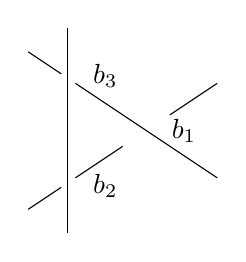
\begin{tikzpicture}
%\clip(-4.5,-1.65) rectangle (4.5, 1.65);


\draw (-4,1) -- (-3.58, 0.72);
\draw (-3.4, 0.6) -- (-1.6,-.6);
\draw (-4, -1) -- (-3.58, -0.72);
\draw (-3.4, -0.6) -- (-2.8, -0.2);
\draw (-2.2, 0.2) -- (-1.6, 0.6);


\draw (-3.5, -1.3) -- (-3.5, 1.3);

\node [below, right] at (-3.3, -0.7) {$b_2$};
\node [above, right] at (-3.3, 0.7) {$b_3$};
\node [right] at (-2.3,0) {$b_1$};
\end{tikzpicture} 
\caption{Typ B}
\end{subfigure}
\begin{subfigure}[t]{0.4\linewidth}\centering
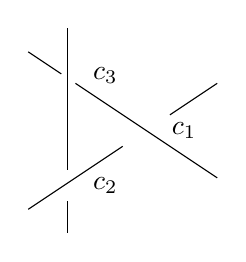
\begin{tikzpicture}
%\clip(-4.5,-1.65) rectangle (4.5, 1.65);


\draw (-4,1) -- (-3.58, 0.72);
\draw (-3.4, 0.6) -- (-1.6,-.6);
\draw (-4, -1) -- (-2.8, -0.2);
\draw (-2.2, 0.2) -- (-1.6, 0.6);


\draw (-3.5, -1.3) -- (-3.5, -0.9);
\draw (-3.5, -0.5) -- (-3.5, 1.3);
\node [below, right] at (-3.3, -0.7) {$c_2$};
\node [above, right] at (-3.3, 0.7) {$c_3$};
\node [right] at (-2.3,0) {$c_1$};
\end{tikzpicture}
\caption{Typ C}
\end{subfigure}
\caption{Typy stěn ohraničených třemi a méně hranami.} \label{stenyobr}
\end{figure}

Stěna s jednou hranou by v diagramu odpovídala smyčce, ty jsou ovšem podle předpokladu už odstraněny rozmotáním.

Možné stěny s dvěma a třemi hranami jsou zobrazené na obrázku~\ref{stenyobr}.

Stěna se dvěma hranami, která není rozmotatelná druhým Reidemeisterovým pohybem, musí v diagramu odpovídat typu A. Všimněme si, že rozpojením křížení $a_1$ i $a_2$ buď ve vertikálním, nebo horizontálním směru vznikne smyčka. Volbou křížení $a_1$ nebo $a_2$ je tedy zaručeno, že jeden syn má po rozmotání nejvýše $n-2$ křížení.

Stěna se třemi hranami v diagramu odpovídá buď typu B, nebo C.

Ve stěně typu B získáme vertikálním rozpojením křížení $b_1$ syna, jenž jde rozmotat druhým Reidemeisterovým pohybem. Jeho diagram tedy bude mít po rozmotání nejvýše $n-3$ křížení.

Ve stěně typu C není rozpojením žádného křížení rozmotání zaručeno. Ovšem rozpojením libovolného křížení získáme jednoho syna se stěnou typu A. Existuje tedy vnuk s nejvýše $n-3$ kříženími.

\subsection{Výsledný algoritmus pro výpočet závorkového polynomu} \label{varianty}
Snažíme se maximalizovat rozmotání u synů, budeme tedy při rozpojování prefeferovat křížení stěn A a B před stěnou C. Dále rozlišíme dvě varianty výsledného algoritmu: \emph{algoritmus A} navíc preferuje křížení $a_i$ před $b_1$,  \emph{algoritmus B} preferuje $b_1$ před $a_i$. Celý postup je shrnut v algoritmu~\ref{alg02:04}.

Původní algoritmus~\ref{alg02:03} s náhodnou volbou křížení a rozmotáváním budeme označovat \emph{algoritmus RND}.

V PD notaci je možné vhodné křížení stěn A, B i C nalézt v lineárním čase vzhledem k $n$, časová složitost tedy zůstává $\mathcal{O}(2^n)$. V následující sekci~\ref{analyza} se pokusíme získat lepší odhady složitosti.

Obě varianty výsledného algoritmu jsou podle úvah v předchozích částech korektní a vždy se zastaví.

\begin{algorithm}[p]

\caption{Výsledný algoritmus pro výpočet závorkového polynomu, varianty A a B.}
\label{alg02:04}

\DontPrintSemicolon

\SetKwData{cross}{křížení}
\SetKwData{dh}{Dh}
\SetKwData{dv}{Dv}
\SetKwData{kk}{k}
\SetKwData{aj}{$a_1$}
\SetKwData{bj}{$b_1$}
\SetKwData{cj}{$c_1$}
\SetKwData{e}{e}
\SetKwData{D}{D}
\SetKwData{lh}{Dh}
\SetKwData{lv}{Dv}
\SetKwData{Hk}{$k_h$}
\SetKwData{Vk}{$k_v$}
\SetKwFunction{Bracket}{Bracket}%
\SetKwData{bracketPoly}{zavorkovýPoly$(t)$}

\SetKwProg{Fn}{Function}{}{end} 


\Fn{\Bracket{$D$}}{
\KwData{Diagram $D$ linku $L$ s $n$ kríženími}
\KwResult{Závorkový polynom v proměnné $A$}
\BlankLine
\If{diagram $D$ nemá žádná křížení}{\KwRet 1}
\BlankLine

rozmotej diagram jako v algoritmu~\ref{alg02:03}

\BlankLine
\If{varianta A} {
\eIf{existuje stěna typu A}
{\cross $\leftarrow$ \aj}
{ \eIf {existuje stěna typu B} {\cross $\leftarrow$ \bj}{ \cross $\leftarrow$ \cj}
}
}
\If{varianta B} {
\eIf{existuje stěna typu B}
{\cross $\leftarrow$ \bj}
{ \eIf {existuje stěna typu A} {\cross $\leftarrow$ \aj}{ \cross $\leftarrow$ \cj}
}
}

\BlankLine
\lh $\leftarrow$ link \D, kde \cross je rozpojeno horizontálně

\lv $\leftarrow$ link \D, kde \cross je rozpojeno vertikálně
\BlankLine

\eIf{v linku \lh vznikla disjunktní kružnice} {\Hk $\leftarrow$ 1} {\Hk $\leftarrow$ 0}
\eIf{v linku \lv vznikla disjunktní kružnice} {\Vk $\leftarrow$ 1} {\Vk $\leftarrow$ 0}
\BlankLine
\bracketPoly $\leftarrow$ $A(-A^2 - A^{-2})^{\Hk} $ \Bracket{\lh} \\  $ \hspace{2.75cm} +A^{-1}(-A^2 - A^{-2})^{\Vk} $ \Bracket{\lv}
\BlankLine
\KwRet \bracketPoly
}

\end{algorithm}


\subsection{Implementace algoritmu}
Algoritmus jsme implementovali v programovacím jazyce Python. 

Práce s diagramem v PD notací s využitím vhodných datových struktur je sice rychlá, ale náročná na rozbor všech možných případů. Ačkoli je tedy samotný algoritmus poměrně přímočarý, délka kódu narostla kvůli nutnosti rozlišení všech případů při rozpojování křížení, rozmotávání diagramu a hledání vhodného křížení.

\section{Analýza složitosti algoritmu}  \label{analyza}
V teto sekci vypočteme horní a dolní odhad algoritmu na výpočet závorkového a Jonesova polynomu. V následující analýze nezáleží, jestli se jedná o variantu A, nebo B.
\subsection{Horní odhad}
Rychlost algoritmu je závislá na počtu křížení $n$ a na míře rozmotávání. Například na diagramu, který je možné absolutně rozmotat použitím prvních dvou Reidemasterových pohybů, poběží nejhůř v kvadratickém čase (příkladem je typ torusových uzlů, viz sekce~\ref{torus}).

\begin{tvrz}
Výpočet Jonesova polynomu založený na algoritmu na výpočet závorkového polynomu~\ref{alg02:04} má časovou složitost  $\mathcal{O}( 2^{0.82 n })$.
\end{tvrz}
\begin{dukaz}
Horní odhad rychlosti algoritmu~\ref{alg02:04} provedeme na příkladu diagramu, v němž dojde pouze k minimálnímu rozmotávání. Nedojde tedy k rozmotání jiných křížení než těch, u kterých je to zaručeno volbou křížení k rozpojení, viz rozbor v sekci~\ref{volba}.
Také v případech, kdy není předchozí volbou křížení zaručena existence stěny typu A, bude existovat pouze stěna typu C, která zaručuje rozmotání pouze u vnuka.

Průběh algoritmu zakreslíme jako binární strom, kde číslo ve vrcholu je počet křížení diagramu. V kořeni máme diagram s $n$ kříženími, v němž rozmotáme křížení stěny C, takže jeho synové jsou diagramy s $n-1$ kříženími a obsahují stěnu typu A. Jejich synové budou diagramy velikosti $n-2$ a $n-3$.
V lichých hladinách stromu má tedy vrchol syny o jedno křížení menší, v sudých hladinách je jeden syn o dvě křížení menší.

\begin{forest}
  [n[n-1[n-2[n-3[n-4[...][...]][n-5[...][...]]][n-3[...][...]]][n-3[n-4[n-5[...][...]][n-6[...][...]]][n-4[...][...]]]][n-1[n-2[...][...]][n-3[...][...]]]]
\end{forest}

Získali jsme rekurentní rovnici na počet operací výpočtu závorkového polynomu diagramu velikosti $n$

$$T(n) = 2 T(n-2) + 2 T(n-3) + C_L n + 2 C_L (n-1).$$

Člen $C_L n + 2 C_L (n-1)$, kde $C_L$ je konstanta, vyjadřuje, že na rozdělení každého diagramu na syny (rozmotání a volba křížení) je potřeba lineární počet operací vzhledem k počtu křížení.

Rekurenci je možné řešit pomocí vytvořujících funkcí a rozkladu na parciální zlomky. Výpočtem získáme vzorec
$$ T(n) \approx C_1 2^{0.82 n } + C_2 n 2^{0.09 n } + C_3 2^{0.09 n } + C_4 n + C_5 ,  $$

kde $C_i$ jsou jisté konstanty.

Z vzorce plyne, že $ T(n)= \mathcal{O}( 2^{0.82 n })  $.

Podle sekce~\ref{jones} je na výpočet Jonesova polynomu ze závorkového polynomu potřeba pouze lineární počet operací. Dohromady má tedy náš výpočet Jonesova polynomu časovou složitost $\mathcal{O}( 2^{0.82 n })$.
\end{dukaz}

\subsection{Dolní odhad}

\begin{tvrz} \label{dolni}
Výpočet Jonesova polynomu založený na algoritmu na výpočet závorkového polynomu~\ref{alg02:04} má časovou složitost  $\Omega(2^{0.75 n})$.
\end{tvrz}

\begin{dukaz}
Provedeme analýzu průběhu algoritmu~\ref{alg02:04} na linku s diagramem, který vznikne z diagramu Borromeovských kruhů přidáváním kružnic. Kružnici přidáváme tak, aby vždy protla dva další kruhy celkem ve čtyřech bodech a upravíme křížení, aby vzniklý diagram byl alternující, tj. aby se střídala křížení vedená zdola a shora, viz obrázek~\ref{borro}. Diagram složený z $k$ kružnic označíme $B_k$.

\begin{figure}[h]  

\centering 
\begin{subfigure}[t]{0.4\linewidth}\centering
\begin{tikzpicture}[scale=0.5]
\begin{knot}[
%  draft mode=crossings,
  flip crossing/.list={3,4}
]
\strand (1.5,0) circle[radius=2cm];
\strand (-1.5,0) circle[radius=2cm];
\strand (0,{1.5*sqrt(3)}) circle[radius=2cm];
\strand[white] (0,{-1.5*sqrt(3)}) circle[radius=2cm];
\end{knot}
\end{tikzpicture} 
\caption{Borromeovské kruhy} 
\end{subfigure}
\begin{subfigure}[t]{0.4\linewidth}\centering
\begin{tikzpicture}[scale=0.5]
\begin{knot}[
% draft mode=crossings,
  flip crossing/.list={8, 7, 4,12, 2,11}
]
\strand (1.5,0) circle[radius=2cm];
\strand(-1.5,0) circle[radius=2cm];
\strand (0,{1.5*sqrt(3)}) circle[radius=2cm];
\strand[blue] (0,{-1.5*sqrt(3)}) circle[radius=2cm];
\strand[blue] (3,{1.5*sqrt(3)}) circle[radius=2cm];
\end{knot}
\end{tikzpicture}
\caption{Přidání dvou kružnic}
\end{subfigure}
\caption{Vznik diagramu $L$ z důkazu tvrzení~\ref{dolni}.} \label{borro}
\end{figure}  


Diagram $B_k$ má $4k-6$ křížení, můžeme tedy tímto způsobem získat diagram s počtem křížením větším než libovolné $n$. Každá stěna diagramu $B_k$ je typu C.

\begin{figure}[p] \centering
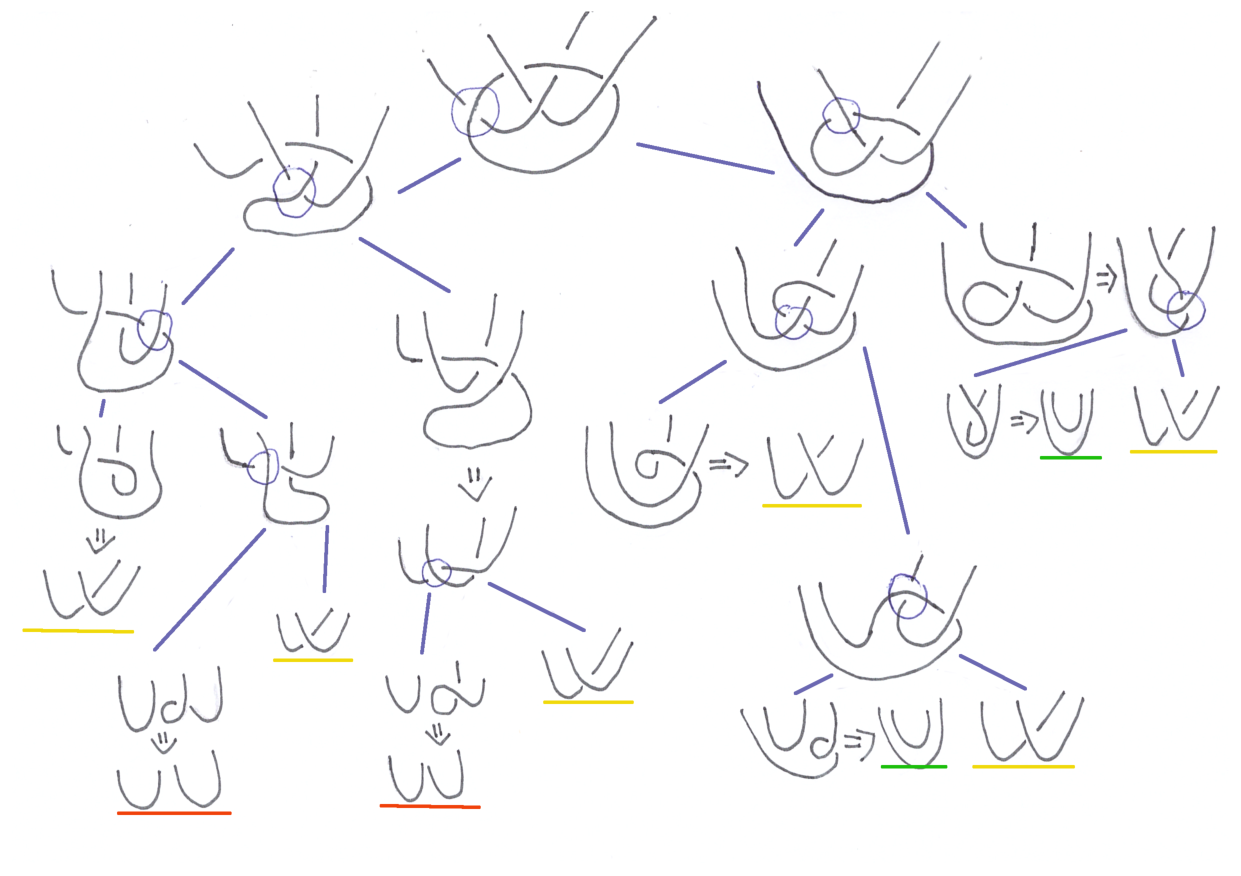
\includegraphics[scale=0.5]{../img/horniodhad}
\caption{Průběh algoritmu na diagramu $B_k$.} \label{prubehhorni}
\end{figure}

Na obrázku~\ref{prubehhorni} je znázorněn strom s průběhem algoritmu na diagramu $B_k$ takový, že jsou postupně odstraňovány krajní kružnice. V kořeni se nachází úsek diagramu obsahující nějakou krajní kružnici. Zakroužkováním je označeno křížení, které bylo vybráno k rozpojení (volba křížení odpovídá variantám A i B a samozřejmě i RND). Šipkou je znázorněno, pokud dojde k rozmotání diagramu. Žlutě podtržení potomci jsou diagramy $B_{k-1}$. Červeně a zeleně podržení potomci jsou synové diagramu $B_{k-1}$, jak je vidět na obrázku~\ref{rozdvojeni}.

\begin{figure}[p] \centering
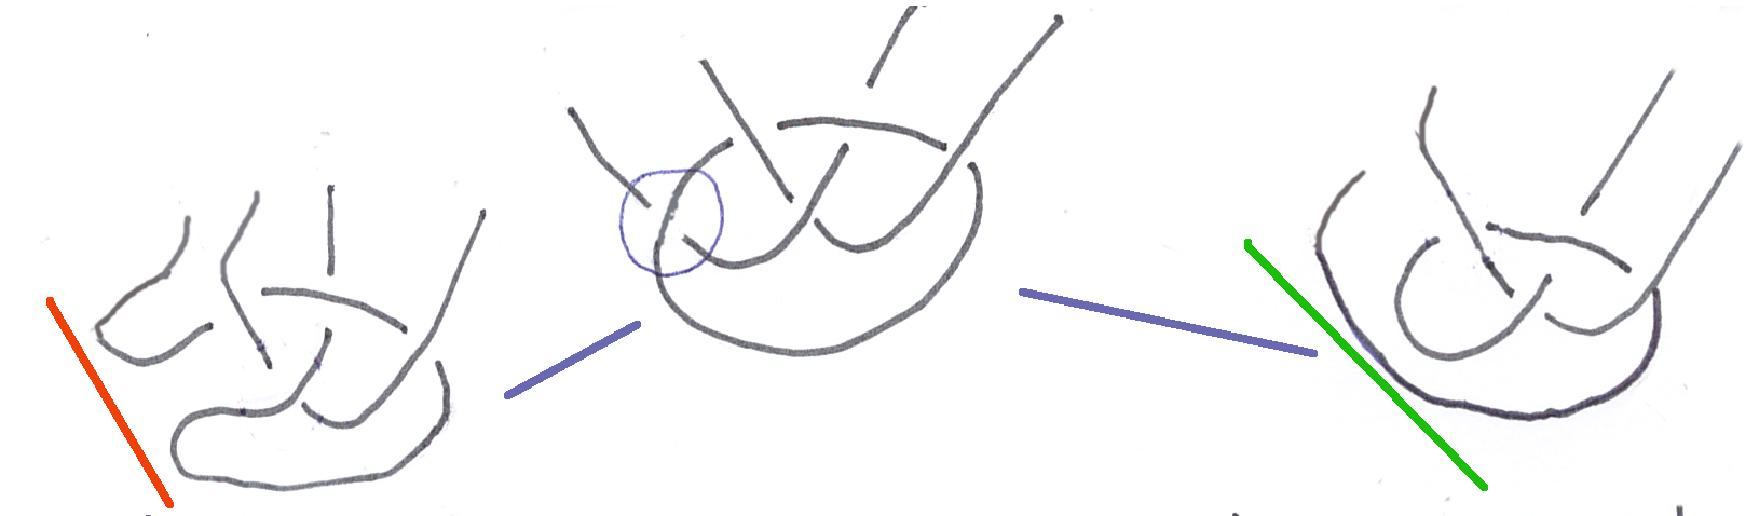
\includegraphics[scale=0.5]{../img/rozdvojeni}
\caption{Synové diagramu $B_{k-1}$.}  \label{rozdvojeni}
\end{figure}

Dohromady tedy z diagramu $B_k$ rozpojováním vznikne šest diagramů $B_{k-1}$ a čtyři synové $B_{k-1}$. Výpočet závorkového polynomu diagramu $B_k$ je tedy těžký alespoň jako výpočet polynomu osmi diagramů $B_{k-1}$. 

Časová složitost algoritmu na diagramu s $n$ kříženími splňuje rekurenci
$$ T(n) = 8T(n-4) + C_1 n + C_0  $$
pro jisté konstanty $C_0$, $C_1$.

Z toho plyne, že $T(n) = \Omega(8^{\frac{n}{4}})  =  \Omega(2^{0.75 n})$. \\

Na výpočet Jonesova polynomu ze závorkového polynomu je potřeba pouze lineární počet operací, tedy i výpočet Jonesova polynomu má časovou složitost $\Omega(2^{0.75n})$.
\end{dukaz}
